%%%%%%%%%%%%%%%%%%%%%%%%%%%%%%%%%%%%%%%%%%%%%%%%%%%%%%%%%%%%%%%
%
% Welcome to Overleaf --- just edit your LaTeX on the left,
% and we'll compile it for you on the right. If you open the
% 'Share' menu, you can invite other users to edit at the same
% time. See www.overleaf.com/learn for more info. Enjoy!
%
%%%%%%%%%%%%%%%%%%%%%%%%%%%%%%%%%%%%%%%%%%%%%%%%%%%%%%%%%%%%%%%


% Inbuilt themes in beamer
\documentclass[15pt]{beamer}

% Theme choice:
\usetheme{CambridgeUS}

% Title page details: 
\title{Assignment-8} 
\author{Shivanshu  Ai21btech11027}
\date{May 29, 2022}


\begin{document}
    \maketitle
    
    \begin{frame}{Question}
        \textbf{Papoulis book exercise 6}\\
        \large \noindent Q-39 The random variable x and y are independent, x is $N(0,\sigma^2)$. and y is uniform in the interval $(0.\pi)$. Show that if $z = x + a cosy$ , then \\
        \begin{center}
             $f_z(z) = \dfrac{1}{\pi\sigma\squareroot{2\pi}}$
        \end{center}
       
    \end{frame}
    \begin{figure}[h]
        \centering
        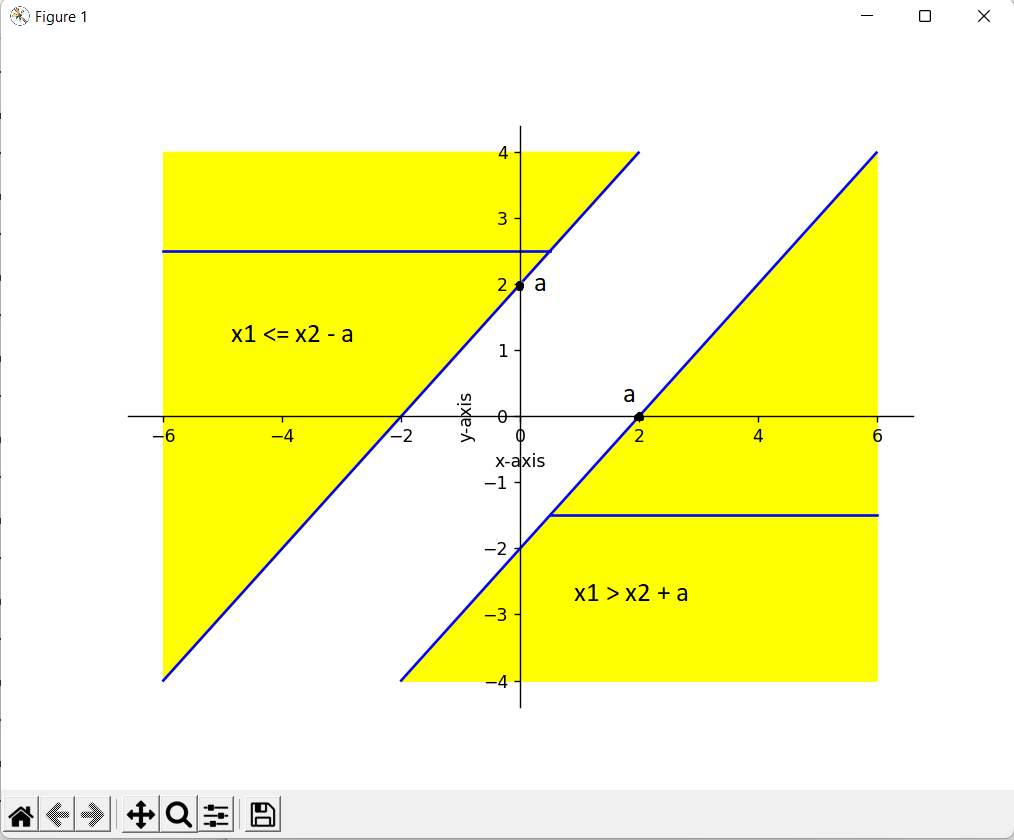
\includegraphics[width=\columnwidth]{fig.jpg}
        \caption{fig. P5-47}
        \label{fig.}
    \end{figure}
    \begin{frame}{Solution}
     From the assumption it follows that \\
     \vspace{2mm}
     $g'(-x) = -g'(x)$ \hspace{5mm} $g"(x) \geq 0$ \hspace{5mm} $f(x - \eta) = f(\eta - x)$ \\
     \vspace{2mm}
     Hence, if $I(a) = E{g(x - a)}$, then \\
     \vspace{2mm}
     $I'(a) = - \int_{-\infty}^{ \infty} g'(x - a)f(x) dx$  \hspace{10mm} $I'(\eta) = 0$ \\
     \vspace{2mm}
     $I"(a) = \int_{-\infty}^{ \infty} g"(x - a)f(x) dx \geq 0$ \hspace{10mm} all a \\
     \vspace{2mm}
     Hence, I(a) is minimum for $a = \eta$.
    \end{frame}
\end{document}
